\thispagestyle{empty}

\chapter{Real-Time Localization System for Autonomous Vehicles}
\thispagestyle{empty}
\label{cpt:localization}

This chapter focuses on the real-time LiDAR localization system. With the foundational point cloud map established, we can match current laser scan data with the map to determine the vehicle's position, which is then fused with IMU and other sensor data using filters \cite{Wang2017}. However, point cloud localization doesn't directly provide physical world coordinates like RTK does - it first requires an approximate initial position to guide the point cloud registration algorithm toward convergence. Consequently, point cloud localization presents some unique logical challenges in practical applications. Using the point cloud map constructed in the previous chapter, this chapter demonstrates the implementation of point cloud localization and presents a real-time localization solution based on a Kalman filter.

\includepdf[width=\textwidth]{art/ch10.pdf}

\section{Design Scheme for Point Cloud Fusion Localization}  
Before designing the overall algorithm flow, let us first examine the characteristics of various sensor inputs.

Compared to traditional integrated navigation systems, high-precision localization for autonomous vehicles primarily incorporates an additional input source: LiDAR-based localization. Traditional RTK-IMU integrated navigation systems are less suitable for scenarios like campuses due to the inherent signal quality limitations of RTK. As readers may observe from the NCLT dataset, RTK signals often exhibit instability—such as jitter or dropout—in many areas. On the other hand, the point cloud map constructed in the previous chapter provides an excellent representation of the 3D structure of static environments. Most large-scale scenes, such as buildings, do not change frequently, making point cloud localization a reliable positioning source. Previous chapters of this book have extensively discussed methods for registering scan point clouds with map point clouds. This chapter will employ the NDT method for registration and ultimately integrate the results into a Kalman filter.

\begin{figure}[!htp]  
	\centering  
	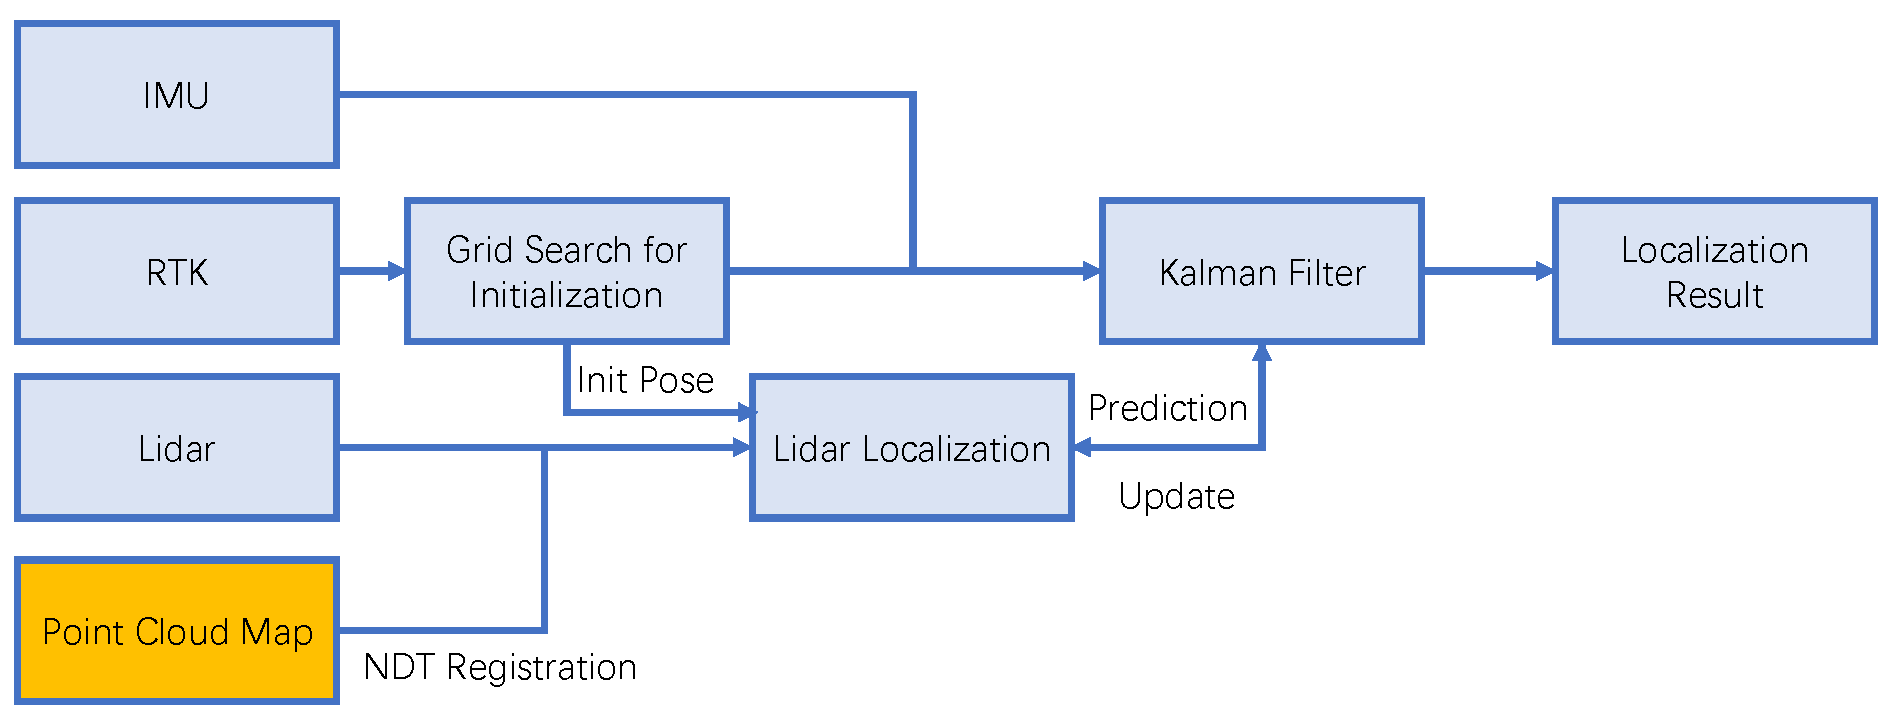
\includegraphics[width=0.8\textwidth]{resources/localization/framework}  
	\caption{Algorithm framework for point cloud fusion localization}  
	\label{fig:localization-framework}  
\end{figure}  

From a fusion perspective, point cloud fusion localization can adopt either an error-state Kalman filter (similar to traditional integrated navigation) or pose graph optimization (like modern SLAM systems). Generally, the Kalman filter approach is simpler to design and implement, often yielding smoother results. However, it may converge to incorrect solutions, leading to localization drift that is difficult to correct. In contrast, graph optimization methods facilitate the detection of discrepancies between various factors and the estimated state, enabling logical handling of anomalies—though ensuring smoothness in localization is more challenging (unless manual marginalization, as in Chapter~\ref{cpt:ins}, is performed, or optimization libraries like GTSAM with built-in marginalization are used).  

First, let us examine the overall algorithm framework (see Fig.~\ref{fig:localization-framework}). This chapter demonstrates a Kalman filter-based localization solution. Since the principles of the Kalman filter have already been detailed in Chapter~\ref{cpt:ins}, the focus here will be on the fusion of point cloud localization with the Kalman filter.  

Point cloud localization requires an initial vehicle position for search, so we design an initialization procedure. When the filter has not yet computed its position, the first valid RTK signal is used to constrain the search range for point cloud localization. Additionally, since the RTK data in the NCLT dataset lacks attitude information, a grid search is employed to determine the vehicle's orientation. Once the Kalman filter converges, its predicted value serves as the initial guess for point cloud registration\footnote{Alternatively, the point cloud localization could predict the next LiDAR pose based on historical poses, improving system decoupling and simplifying debugging.}.  

At the point cloud localization level, we use the partitioned point clouds from the previous chapter. Since the point clouds were divided into 100m×100m grid cells earlier, this chapter loads a 3×3 grid (nine cells) around the vehicle. To prevent frequent loading/unloading when the vehicle moves near grid boundaries, an unloading threshold (set to three cells in our implementation) is applied—only cells beyond this range are unloaded.

\section{Algorithm Implementation}  
Now we proceed to implement the algorithm described earlier. The code implementation in this chapter reuses portions of the filter from Chapter~\ref{cpt:ins} and the IMU processing code from Chapter~\ref{cpt:tightly-lio}.  

\subsection{RTK Initialization Search}  
Following the algorithm flow outlined previously, the system cannot perform point cloud localization until it receives the first valid RTK signal, as the vehicle's position in the map is unknown. Upon receiving the first valid RTK signal, we conduct a \textbf{grid search} around it. Our designed search process primarily determines the vehicle's initial heading angle by employing a multi-resolution matching method similar to that used in loop detection (Chapter~\ref{cpt:tightly-lio}).  

\begin{lstlisting}[language=c++,caption=/ch10/fusion.cc]  
bool Fusion::SearchRTK() {  
	// Since RTK lacks attitude, we must search within an angular range  
	std::vector<GridSearchResult> search_poses;  
	LoadMap(last_gnss_->utm_pose_);  
	
	/// RTK provides no orientation, so we scan angles at fixed intervals  
	double grid_ang_range = 360.0, grid_ang_step = 10;  // Angular search range and step  
	for (double ang = 0; ang < grid_ang_range; ang += grid_ang_step) {  
		SE3 pose(SO3::rotZ(ang * math::kDEG2RAD), Vec3d(0, 0, 0) + last_gnss_->utm_pose_.translation());  
		GridSearchResult gr;  
		gr.pose_ = pose;  
		search_poses.emplace_back(gr);  
	}  
	
	LOG(INFO) << "grid search poses: " << search_poses.size();  
	std::for_each(std::execution::par_unseq, search_poses.begin(), search_poses.end(),  
	[this](GridSearchResult& gr) { AlignForGrid(gr); });  
	
	// Select the best-matching result  
	auto max_ele = std::max_element(search_poses.begin(), search_poses.end(),  
	[](const auto& g1, const auto& g2) { return g1.score_ < g2.score_; });  
	LOG(INFO) << "max score: " << max_ele->score_ << ", pose: \n" << max_ele->result_pose_.matrix();  
	if (max_ele->score_ > rtk_search_min_score_) {  
		LOG(INFO) << "Initialization succeeded, score: " << max_ele->score_ << ">" << rtk_search_min_score_;  
		status_ = Status::WORKING;  
		
		/// Reset filter state  
		auto state = eskf_.GetNominalState();  
		state.R_ = max_ele->result_pose_.so3();  
		state.p_ = max_ele->result_pose_.translation();  
		state.v_.setZero();  
		eskf_.SetX(state, eskf_.GetGravity());  
		
		ESKFD::Mat18T cov;  
		cov = ESKFD::Mat18T::Identity() * 1e-4;  
		cov.block<12, 12>(6, 6) = Eigen::Matrix<double, 12, 12>::Identity() * 1e-6;  
		eskf_.SetCov(cov);  
		
		return true;  
	}  
	
	init_has_failed_ = true;  
	last_searched_pos_ = last_gnss_->utm_pose_;  
	return false;  
}  

void Fusion::AlignForGrid(sad::Fusion::GridSearchResult& gr) {  
	/// Multi-resolution NDT  
	pcl::NormalDistributionsTransform<PointType, PointType> ndt;  
	ndt.setTransformationEpsilon(0.05);  
	ndt.setStepSize(0.7);  
	ndt.setMaximumIterations(40);  
	
	ndt.setInputSource(current_scan_);  
	auto map = ref_cloud_;  
	
	CloudPtr output(new PointCloudType);  
	std::vector<double> res{10.0, 5.0, 4.0, 3.0};  
	Mat4f T = gr.pose_.matrix().cast<float>();  
	for (auto& r : res) {  
		auto rough_map = VoxelCloud(map, r * 0.1);  
		ndt.setInputTarget(rough_map);  
		ndt.setResolution(r);  
		ndt.align(*output, T);  
		T = ndt.getFinalTransformation();  
	}  
	
	gr.score_ = ndt.getTransformationProbability();  
	gr.result_pose_ = Mat4ToSE3(ndt.getFinalTransformation());  
}  
\end{lstlisting}



